\section{Removing Vertices}
\label{sect:removing-vertices}

same distinguishment: internal vs external, reverses the insert inside/outside.



\paragraph{Removing Internal Vertices}

can only remove internal if degree 3. if higher degree we would create hole. need to flip edges first.\cref{sect:flipping-edges}

\begin{figure}[H]
	\centering
	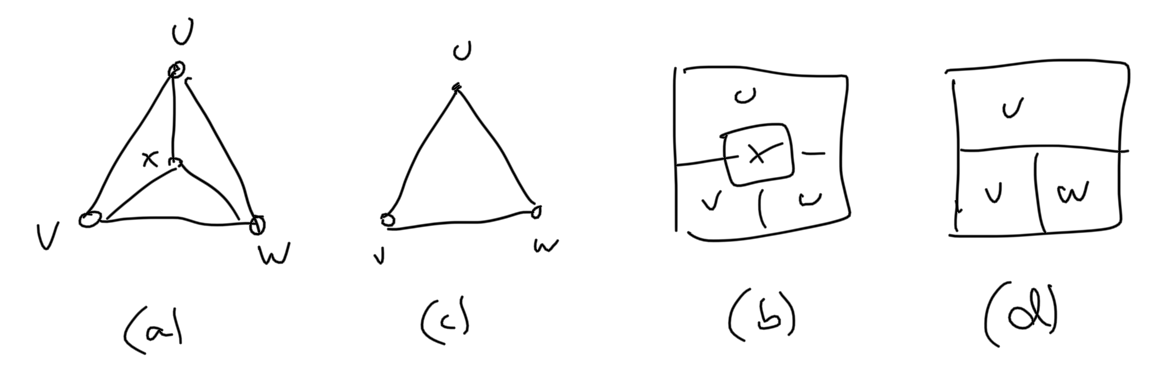
\includegraphics[height=30mm]{Resources/RemoveInternalVertex.png}
	\caption{A cluster graph and a polygonal dual thereof, before (a, b) and after (c, d) removing the internal vertex $x$ with degree 3.}
	\label{fig:remove-internal-vertex-example}
\end{figure}

\begin{itemize}
	\item compute boundary (path) with the three incident faces: $u$-$x$, $v$-$x$, $w$-$x$
	\item contract these boundaries into single-edge-boundaries (why is this possible?)
	\item we then have a plain triangle
	\item replace triangle with single point in its barycenter
\end{itemize}

 % either hack, assign area to another face by removing one of three boundaries. or: contract boundaries until they are 1 long each -> face is triangle. then place new vertex in barycenter + connect.



\paragraph{Removing External Vertices}

when removing vertices on the outer face along with its incident edges, we must ensure that the graph remains 2-connected afterwards.

as long as that's given, removing such a vertex is easy though. we just remove the respective face's boundary with the outer face.

\begin{figure}[H]
	\centering
	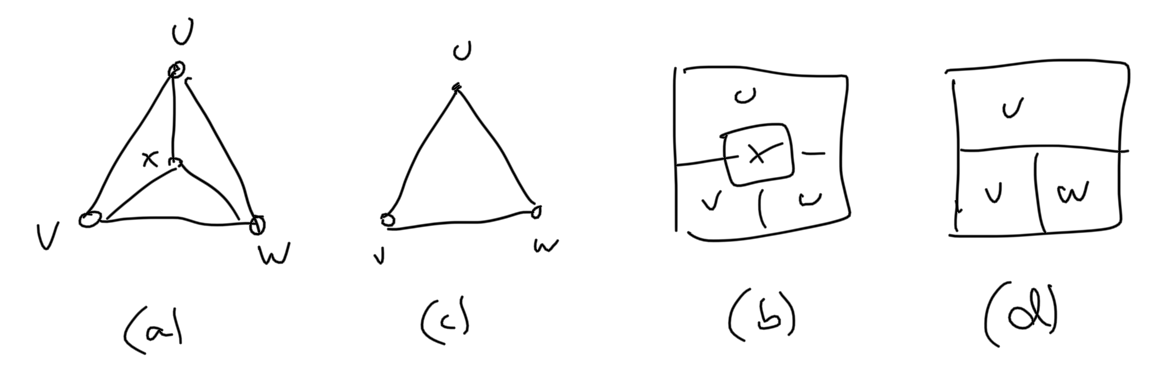
\includegraphics[height=30mm]{Resources/RemoveInternalVertex.png}
	\caption{A cluster graph and a polygonal dual thereof, before (a, b) and after (c, d) removing the vertex $x$ on the outer face.}
	\label{fig:remove-external-vertex-example}
\end{figure}

\begin{itemize}
	\item find boundary of respective face with outer face
	\item remove all internal/subdivision vertices and edges on this path
\end{itemize}
